\documentclass[pdflatex,compress]{beamer}

%\usetheme[dark,framenumber,totalframenumber]{ElektroITK}
\usetheme[darktitle,framenumber,totalframenumber]{ElektroITK}

\usepackage{graphicx}

\title{METODE NUMERIK}
\subtitle{Interpolasi dan Regresi}

\author{Mifta Nur Farid}

\begin{document}

\maketitle

\section{Pengantar}

\begin{frame}
	\frametitle{Pengantar}
	\begin{itemize}
		\item Misalkan diketahui tabel hasil pembacaan suhu dari suatu reaksi kimia sebagai berikut
		\begin{center}
			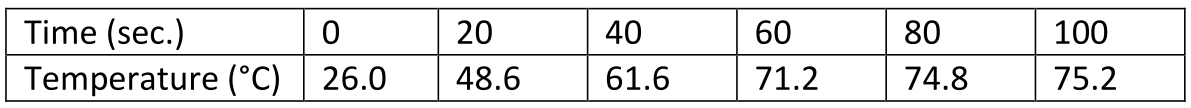
\includegraphics[width=0.8\linewidth]{img/img01}
		\end{center}
		\item Kemudian linear plot dari data di atas adalah:
		\begin{center}
			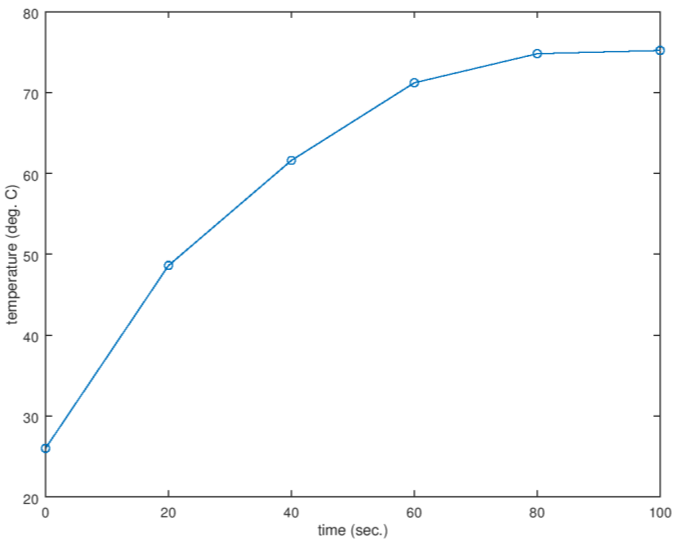
\includegraphics[width=0.5\linewidth]{img/img02}
		\end{center}
	\end{itemize}
\end{frame}

\begin{frame}{Pengantar}
	\begin{itemize}
		\item Berdasarkan data tersebut, jika kita memerlukan suhu reaksi saat detik ke 50, bagaimana cara kita memperoleh data tersebut?
		\item Cara yang dapat kita lakukan adalah melakukan \textbf{interpolasi}.
		\item Kita akan mempelajari interpolasi dan regresi.
	\end{itemize}
\end{frame}

\begin{frame}
	\frametitle{Sub-CPMK}
	Mahasiswa mampu menentukan akar-akar dari persamaan non linear secara numerik
\end{frame}

\begin{frame}
	\frametitle{Bahan Kajian}
	\begin{enumerate}
		\item Metode iterasi sederhana;
		\item Metode Newton-Raphson;
		\item Metode bagi dua/ biseksi;
		\item Metode Regula-Falsi;
		\item Metode Secant.
	\end{enumerate}
\end{frame}

\end{document}
